\chapter*{Epilogue:
	Creating your own Mad Map}

\begin{figure}[h]
\centering
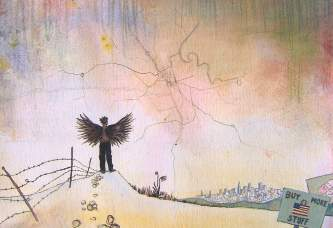
\includegraphics[height=12cm]{TeX_files/5-0.png}
\caption{Artist: Jacks McNamara}
\label{2-0}
\end{figure}


As you made your way through this book did you check off any items or answer the questions? Below you’ll find all the questions repeated--you might want to write your answers here, including any of the items you checked, so you have them organized in one place. Afterward, think about how you would like to represent your answers: lists, drawings, a vision board, a wall dedicated to mapping, photo maps, a journal, or an essay all are ways community members have used to showcase their map. You can choose the one that best suits your style, or even mix and match.

Once you know how you want to build your map, choose a setting that is right for you. Some people like to answer these questions in private, with a friend, in a group, or with support from our online community. The Icarus Project also offers mad mapping workshops so you can make your map with the help of a skilled facilitator.

We suggest you take it easy, be honest with yourself, honor your feelings, and reach out for support so you can safely recover from any triggers sharing this information may cause.

If you end up adding your own questions, want to anonymously share your map with others, or want to use this guide for a group we’d love your additions to this community project! Email \href{mailto:madmaps@theicarusproject.net}{madmaps@theicarusproject.net} to let us know.


\begin{itemize}  
	\item What does oppression feel like?
	\item In what ways do you experience oppression?
	\item Do you experience daily microaggressions?
	\item Does oppression affect how you feel?
	\item Does oppression affect how you behave?
	\item How does oppression impact your mental, emotional and physical health?
	\item How does your body react to microaggressions?
	\item How does oppression affect the way you perceive yourself?
	\item What are some social consequences of oppression that you experience?
	\item How do you cope with the impact of oppression?
	\item How do you navigate triggering situations?
	\item How can people help you? How can we help each other?
	\item Where can we begin to address oppression in our communities?
	\item What steps can your community take to mitigate oppression? What steps can your community take to mitigate oppression?
\end{itemize}

